\usepackage{xcolor}
\usepackage{afterpage}
\usepackage{pifont,mdframed}
\usepackage[bottom]{footmisc}
\usepackage{minted}

\createsection{\Grader}{Grader di prova}

\newcommand{\inputfile}{\texttt{stdin}}
\newcommand{\outputfile}{\texttt{stdout}}
\makeatletter
\renewcommand{\this@inputfilename}{\texttt{stdin}}
\renewcommand{\this@outputfilename}{\texttt{stdout}}
\makeatother

% % % % % % % % % % % % % % % % % % % % % % % % % % % % % % % % % % % % % % % % % % %
% % % % % % % % % % % % % % % % % % % % % % % % % % % % % % % % % % % % % % % % % % %

Una recente analisi condotta dal CERN ha dimostrato come ai bolognesi piacciano gli edifici rossi.
In particolare, Filippo, anch'esso amante degli edifici rossi, ha deciso di comprare un'appartamento
nella via principale di Bologna.

\begin{figure}[h]
    \centering
    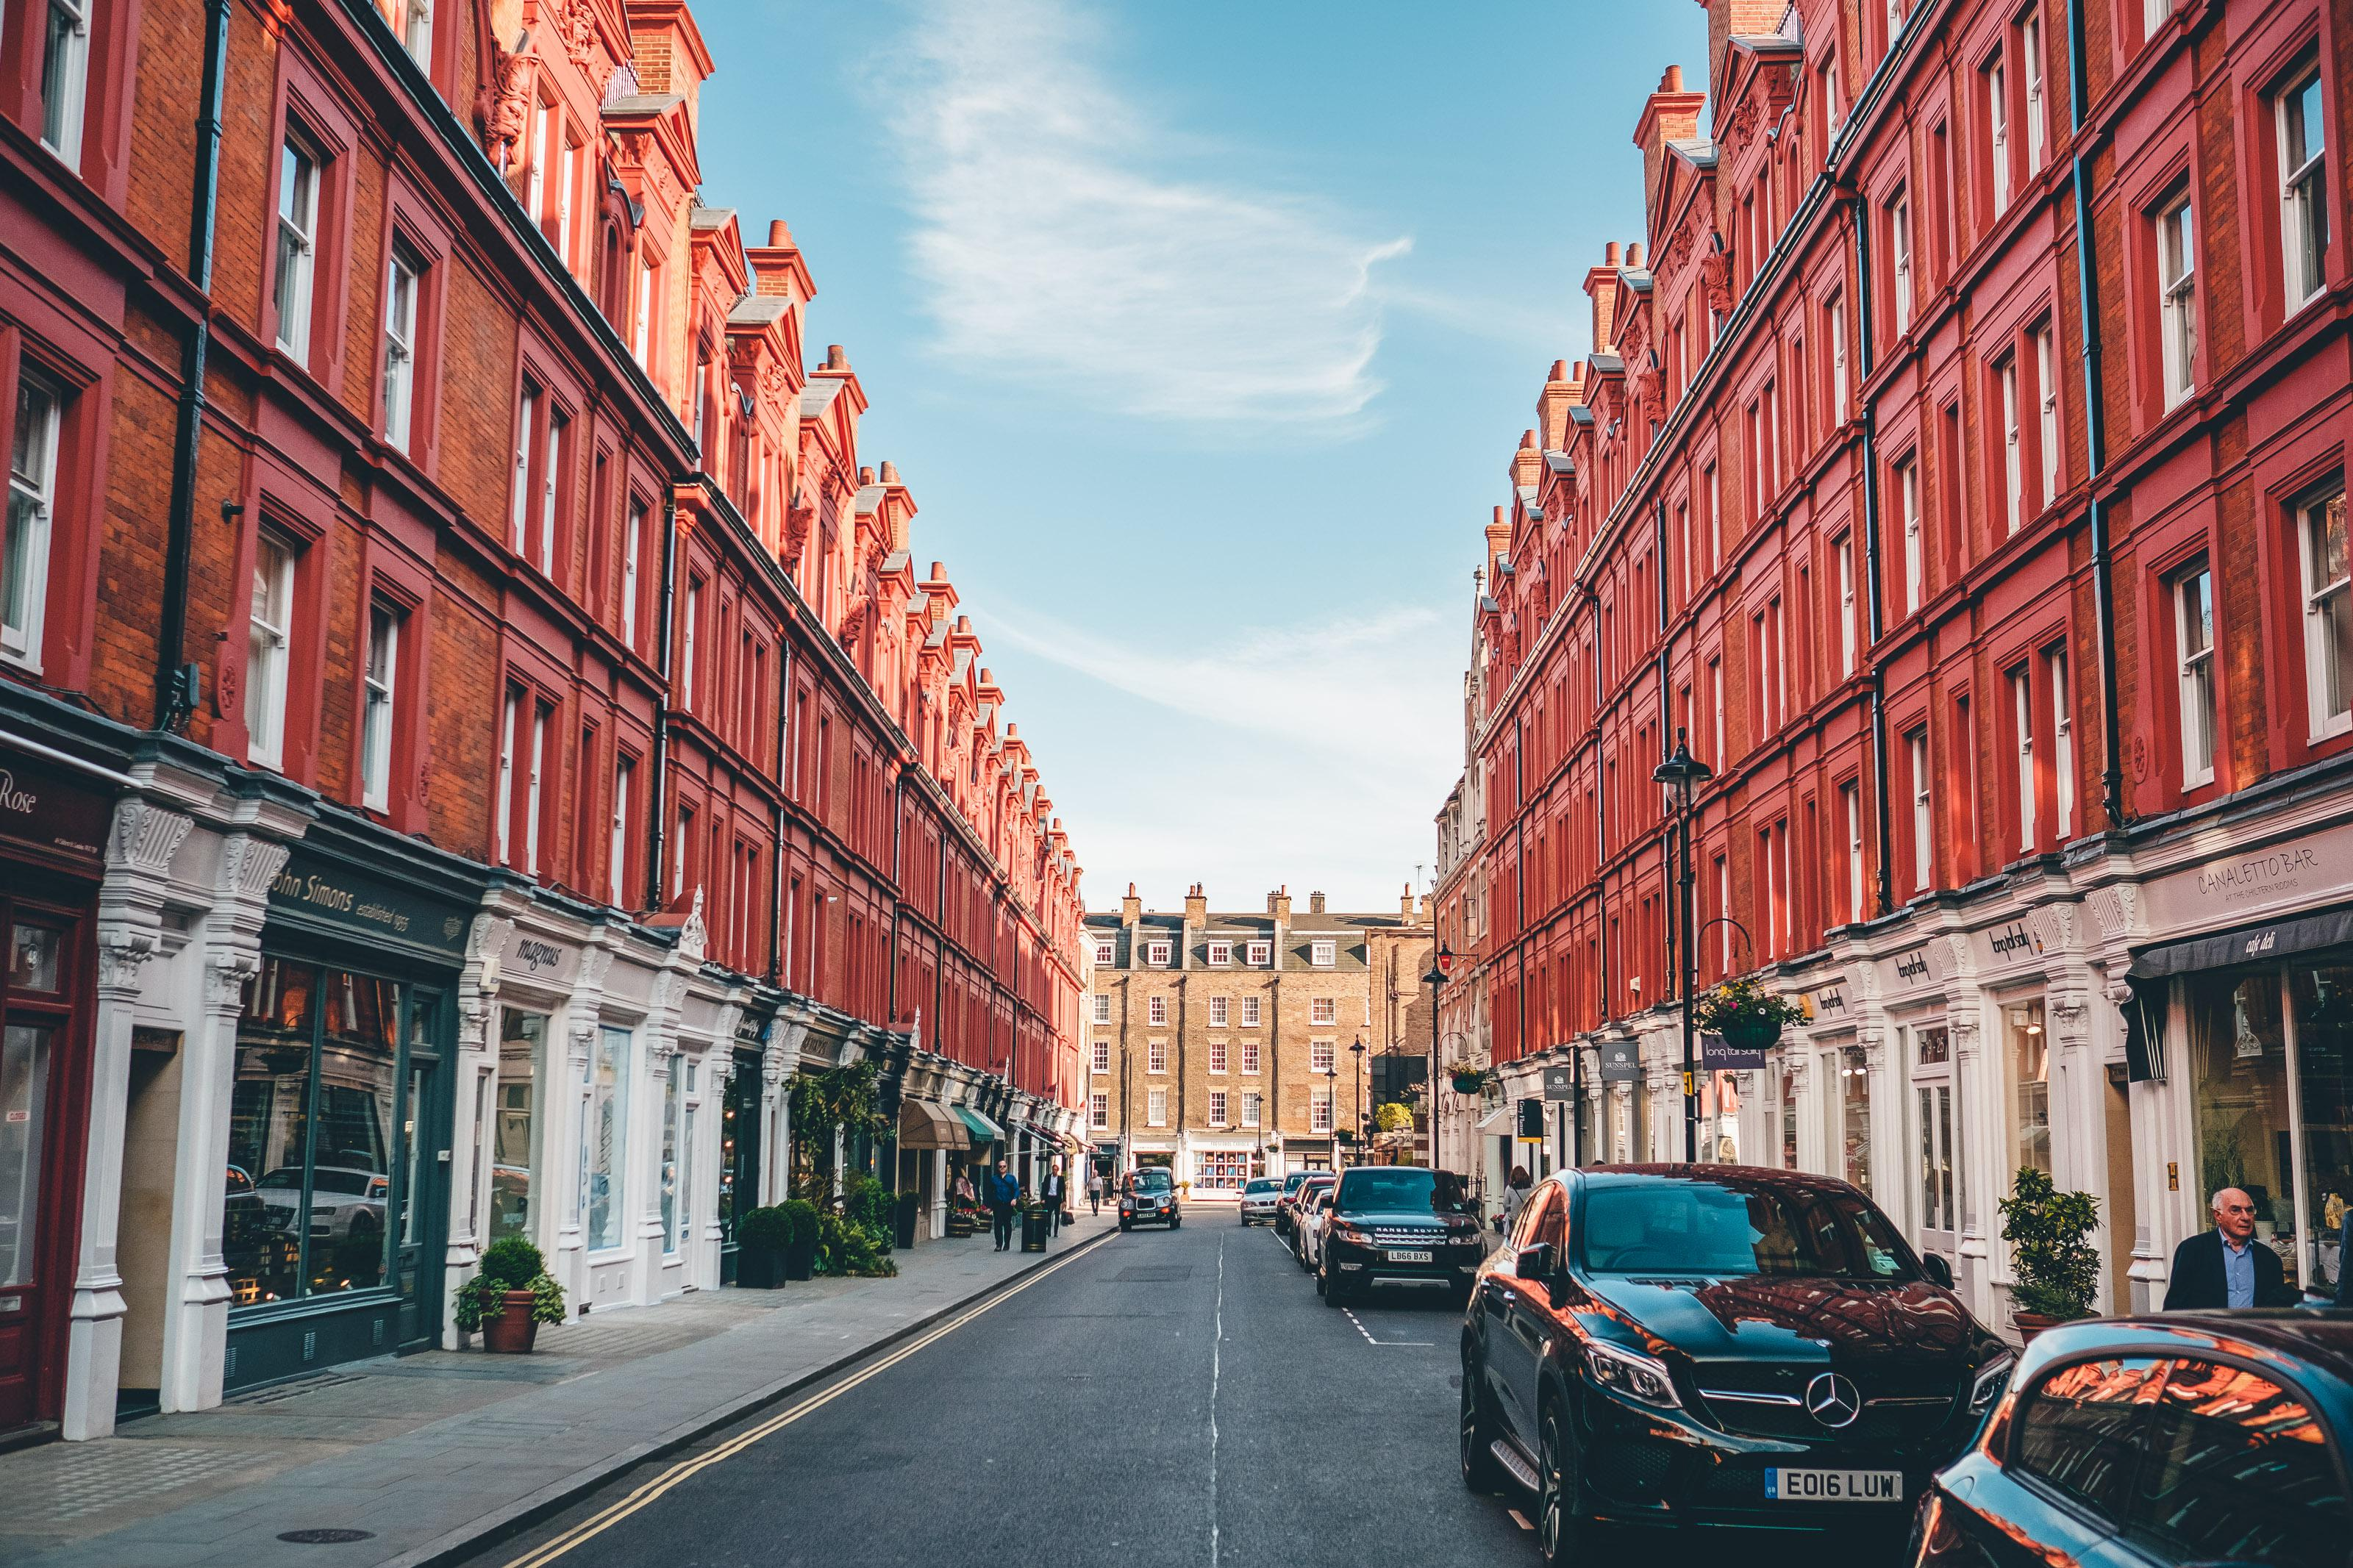
\includegraphics[width=0.5\textwidth]{bologna.jpg}
    \caption{La via principale di Bologna. }
\end{figure}

La via è formata da N abitazioni, dove l'$i$-esimo edificio
è alto $H_i$ metri. Filippo però soffre di vertigini e vuole comprare l'edificio \textbf{più basso} possibile.
Il servizio \textit{Tecnocasa} purtroppo è sotto attacco hacker e non è raggiungibile. Trova quindi l'altezza del palazzo più basso.

% % % % % % % % % % % % % % % % % % % % % % % % % % % % % % % % % % % % % % % % % % %
% % % % % % % % % % % % % % % % % % % % % % % % % % % % % % % % % % % % % % % % % % %

\Implementation

Dovrai sottoporre un unico file, con estensione \texttt{.cpp}.

\begin{warning}
    Tra gli allegati a questo task troverai un template \texttt{bologna.cpp} con un esempio di implementazione.
\end{warning}

Il file di input è composto da $2$ righe:
\begin{itemize}
    \item Riga 1: l'intero N.
    \item Riga 2: gli interi $H_0, H_1, \dots, H_{N-1}$.
\end{itemize}

Il file di output è composto da $1$ righe, contenente la risposta al problema.

% % % % % % % % % % % % % % % % % % % % % % % % % % % % % % % % % % % % % % % % % % %
% % % % % % % % % % % % % % % % % % % % % % % % % % % % % % % % % % % % % % % % % % %

\Constraints

\begin{itemize}[nolistsep, itemsep=2mm]
    \item $1 \le N \le 100\:000$.
    \item $0 \le H_i \le 1\:000\:000$ per ogni $i = 0, \dots,N-1$.
\end{itemize}

% % % % % % % % % % % % % % % % % % % % % % % % % % % % % % % % % % % % % % % % % % %
% % % % % % % % % % % % % % % % % % % % % % % % % % % % % % % % % % % % % % % % % % %

\Scoring

Il tuo programma verrà testato su diversi test case raggruppati in subtask.
Per ottenere il punteggio relativo ad un subtask,
è necessario risolvere correttamente tutti i test che lo compongono.

\begin{itemize}[nolistsep,itemsep=2mm]
    \item \subtask Casi d'esempio.
    \item \subtask Tutti gli $H_i$ sono uguali.
    \item \subtask $N \le 1000$
    \item \subtask Nessuna limitazione aggiuntiva.
\end{itemize}

% % % % % % % % % % % % % % % % % % % % % % % % % % % % % % % % % % % % % % % % % % %
% % % % % % % % % % % % % % % % % % % % % % % % % % % % % % % % % % % % % % % % % % %

\Examples

\begin{example}
    \exmpfile{bologna.input0.txt}{bologna.output0.txt}%
\end{example}

% % % % % % % % % % % % % % % % % % % % % % % % % % % % % % % % % % % % % % % % % % %
% % % % % % % % % % % % % % % % % % % % % % % % % % % % % % % % % % % % % % % % % % %

\Explanation

Nel primo caso di esempio, tra tutti gli edifici quello più basso è quello in posizione $3$, con altezza $2$.
La risposta al problema è quindi $2$.
